\subsection{Implementasi Halaman \textit{Login}}
Halaman ini dapat diakses oleh semua pengguna, baik yang belum terdaftar maupun sudah, dengan pengecualian pengguna tidak dalam keadaan sudah \textit{login}. Halaman ini menampilkan form berisi elemen \textit{input} email dan \textit{password}, dan pengguna dapat mengisi lalu mengklik tombol \textit{login}, dan untuk kasus normal dan alternatif dapat dilihat pada tabel spesifikasi kasus penggunaan \ref{uc01.02}.\\
\indent Tidak ada \textit{view logic} dalam halaman ini. Kode sumber implementasi \textit{back-end} dapat dilihat pada kode sumber \ref{cdbe.01-02}.

\begin{lstlisting}[label=cdbe.01-02,style=php,caption=Kode Sumber Antarmuka Registrasi]
public function showLoginForm(){
	/*Menampilkan halaman login
	  Method : GET */
	return view('auth.login2');
}

public function login(Request $request){
	/*	Setelah klik tombol login,
		masuk ke dalam fungsi ini
		Method : POST */
	$this->validateLogin($request);
	return $this->sendLoginResponse($request);
}

\end{lstlisting}

\begin{figure}[H]
	\centering
	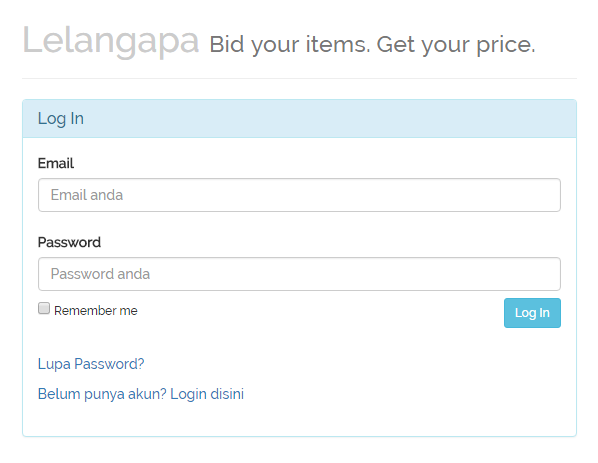
\includegraphics[width=\textwidth]{images/bab4/ui/01-02.png}
	\caption{Halaman Antarmuka }
	\label{ui.01-01}
\end{figure}

